% VLDB template version of 2020-08-03 enhances the ACM template, version 1.7.0:
% https://www.acm.org/publications/proceedings-template
% The ACM Latex guide provides further information about the ACM template

\documentclass[sigconf, nonacm]{acmart}

\usepackage{algorithm,algpseudocode}

%% The following content must be adapted for the final version
% paper-specific
\newcommand\vldbdoi{XX.XX/XXX.XX}
\newcommand\vldbpages{XXX-XXX}
% issue-specific
\newcommand\vldbvolume{14}
\newcommand\vldbissue{1}
\newcommand\vldbyear{2020}
% should be fine as it is
\newcommand\vldbauthors{\authors}
\newcommand\vldbtitle{\shorttitle} 
% leave empty if no availability url should be set
\newcommand\vldbavailabilityurl{URL_TO_YOUR_ARTIFACTS}
% whether page numbers should be shown or not, use 'plain' for review versions, 'empty' for camera ready
\newcommand\vldbpagestyle{plain} 

\begin{document}
\title{Active learning isn't enough: Towards interpretable implicit recommendation for Exploratory Data Analysis}

%%
%% The "author" command and its associated commands are used to define the authors and their affiliations.
\author{David Adams}
\affiliation{%
  \institution{University of Melbourne}
  \streetaddress{Grattan Street Parkville}
  \city{Melbourne}
  \state{Victoria}
  \postcode{3010}
}
\email{david.adams1@student.unimelb.edu.au}

%%
%% The abstract is a short summary of the work to be presented in the
%% article.
\begin{abstract}
Exploratory Data Analysis (EDA) is a critical step in the data science workflow, enabling analysts to uncover patterns, spot anomalies, and test hypotheses. 
\end{abstract}

\maketitle

%%% do not modify the following VLDB block %%
%%% VLDB block start %%%
\pagestyle{\vldbpagestyle}
\begingroup\small\noindent\raggedright\textbf{PVLDB Reference Format:}\\
\vldbauthors. \vldbtitle. PVLDB, \vldbvolume(\vldbissue): \vldbpages, \vldbyear.\\
\href{https://doi.org/\vldbdoi}{doi:\vldbdoi}
\endgroup
\begingroup
\renewcommand\thefootnote{}\footnote{\noindent
This work is licensed under the Creative Commons BY-NC-ND 4.0 International License. Visit \url{https://creativecommons.org/licenses/by-nc-nd/4.0/} to view a copy of this license. For any use beyond those covered by this license, obtain permission by emailing \href{mailto:info@vldb.org}{info@vldb.org}. Copyright is held by the owner/author(s). Publication rights licensed to the VLDB Endowment. \\
\raggedright Proceedings of the VLDB Endowment, Vol. \vldbvolume, No. \vldbissue\ %
ISSN 2150-8097. \\
\href{https://doi.org/\vldbdoi}{doi:\vldbdoi} \\
}\addtocounter{footnote}{-1}\endgroup
%%% VLDB block end %%%

%%% do not modify the following VLDB block %%
%%% VLDB block start %%%
\ifdefempty{\vldbavailabilityurl}{}{
\vspace{.3cm}
\begingroup\small\noindent\raggedright\textbf{PVLDB Artifact Availability:}\\
The source code, data, and/or other artifacts have been made available at \url{\vldbavailabilityurl}.
\endgroup
}
%%% VLDB block end %%%

\section{Introduction}

No one can really agree on a definition of EDA. It is generally accepted that EDA is a process of exploring data to find patterns, anomalies, and relationships. However, the specific techniques and tools used for EDA can vary widely depending on the context and the goals of the analysis.

% what is an insight

But more importantly no one can agree on what an Insight is. Is it a correlation? A trend? A cluster? A outlier? A distribution? A summary statistic? A visualization? A hypothesis? A question? A story? Some people attempt to provide an informal mathematical definition \cite{PDFExtractingTopK} but these are usually inefficient

% active learning is not enough

The most sucessful interactive reccomendation systems such as AIDE (also known as explore by example) \cite{dimitriadouAIDEActiveLearningBased2016}. There are other similar systems such as
AIDE focuses on predicting similar items not what is actually interesting to the user. 

I argue that while we do need to shape the exploration direction based on user feedback, explicit feedback through the ranking of tuples like in AIDE \cite{dimitriadouAIDEActiveLearningBased2016} is no only unecessary but potentially harmful to the analysis process.
Instead I propose that implicit feedback through the analysis of user interactions with the system is a more effective way to guide the exploration process. This is because implicit feedback is more natural and less intrusive than explicit feedback, and it can provide a richer and more nuanced understanding of the user's interests and goals.

Explicit feedback is limited, biased and sparse and it does not always reflect the user's true interests and goals. For example, a user might rank a tuple highly because it is easy to understand, but it might not be particularly interesting or relevant to their analysis. Conversely, a user might rank a tuple lowly because it is difficult to understand, but it might be very interesting or relevant to their analysis.

% One interestingness measure is not enough

From a theoretical perspective, it is clear that no one interestingness measure is enough to capture the full range of insights that an analyst might be interested in. For example, a correlation might be interesting to one analyst, but a cluster might be more interesting to another. A trend might be interesting to one analyst, but an outlier might be more interesting to another. A distribution might be interesting to one analyst, but a summary statistic might be more interesting to another. A visualization might be interesting to one analyst, but a hypothesis might be more interesting to another. A question might be interesting to one analyst, but a story might be more interesting to another.
One of the more formal approaches comes from Hilderman et al who propose a framework for interestingness measures based on the concept of "surprise" \cite{robertj.hildermanInterestingnessFramework2001}.
\cite{robertj.hildermanInterestingnessFramework2001}

The idea that a single interestingness measure has been experimentally validated in the context of EDA \cite{somechPredictingWhatInteresting2019}.

Whilst there has been some work on examining what interestingness measures are applied in EDA \cite{chansonInterestingnessMeasuresExploratory2025a} it fails to 

Due to the wide variety of interetingness measures it is difficult for a benchmark to evaluate all of them or vaious combinations.

% what an EDA system should do

\begin{enumerate}
  \item Keep the human user in the loop as we need to leverage domain knowledge and human intuition.
  \item Not ask the user for explicit feedback 
  \item Provide potential insights in an interpretable way
  \item work on both fast and slow timescales 
  \item be able to work with both small and large datasets
  \item be able to predict users interest on short and long term timescales
  \item be able to explore full data collections autonomously
\end{enumerate}


\section{Methodology}

The first step in creating this system is to evaluate if our system can understand what insight the user is actually interested in. 

As there is no agreed upon definition of EDA or insight it is difficult to evaluate the effectiveness of an EDA system. Given user studies are expensive and time consuming we propose a proxy of the prediction accuracy of the system in predicting future tuples a user will access multiple time steps into the future. 

We propose a simple system that predicts tuples a user will be interested in based on the interestingness of their past queries.

Broadly speaking there are two classes of interestingness measures, those that work on mined patterns and those that work on summarised data \cite{robertj.hildermanKnowledgeDiscoveryMeasures2001}. 

\textbf{Interestingness Contribution Scheme.} To leverage both classes of interestingness measures, we combine association rule mining with database summarization using a novel interestingness contribution scheme. Association rules of the form $X \implies Y$ are mined from query results using standard measures (support, confidence, lift). Simultaneously, we apply Bottom Up Summarization (BUS) \cite{chandola_summarizationcompressing_2007} to identify representative itemsets from closed frequent patterns, creating summary rows with derived count fields that enable diversity-based interestingness measures.

For each tuple $t$, we compute a combined interestingness score as:
\[
I(t) = \alpha \sum_{r\in R} \frac{I(r)}{|X_r \cup Y_r|} f_r(t) + \beta \sum_{s\in S} \frac{I(s)}{|s|} g_s(t)
\]
where $f_r(t)$ and $g_s(t)$ are indicator functions for whether tuple $t$ matches rule $r$ or belongs to summary $s$, respectively. The normalization by pattern size prevents longer patterns from dominating the score, while parameters $\alpha$ and $\beta$ control the relative influence of association rules versus summaries.

Our experiments are primarily conducted on the Sloan Digital Sky Survey (SDSS) dataset \cite{york_sloan_2000}. The SDSS dataset is a large, publicly available dataset that contains information about millions of celestial objects. The dataset is well-suited for our experiments because it is large, complex, and contains a wide variety of data types.

Relying on just the query results to determine what the user is interested in is not enough. For example, if a user queries for all galaxies with a redshift greater than 0.5, they might be interested in the distribution of redshifts, the correlation between redshift and other properties, or the presence of outliers. However, they might also be interested in other properties of galaxies that are not directly related to redshift, such as their morphology or environment.

One might assume there is some kind of linear or superlinear decay in the overlap in tuples between sucessive results sets. However, in practice this is not the case. The overlap between sucessive result sets is often very small, and can even be zero. This is because users often change their queries in ways that are not predictable. For example, a user might start by querying for all galaxies with a redshift greater than 0.5, but then they might change their query to look for all galaxies with a redshift greater than 0.6. This change in query can result in a completely different set of results, with little or no overlap with the previous set.
Conversely if the user makes a small change to their query, such as changing the redshift threshold from 0.5 to 0.51, the overlap between the two result sets can be very high. This is because the two queries are very similar, and they are likely to return many of the same tuples.



\begin{figure}
\centering
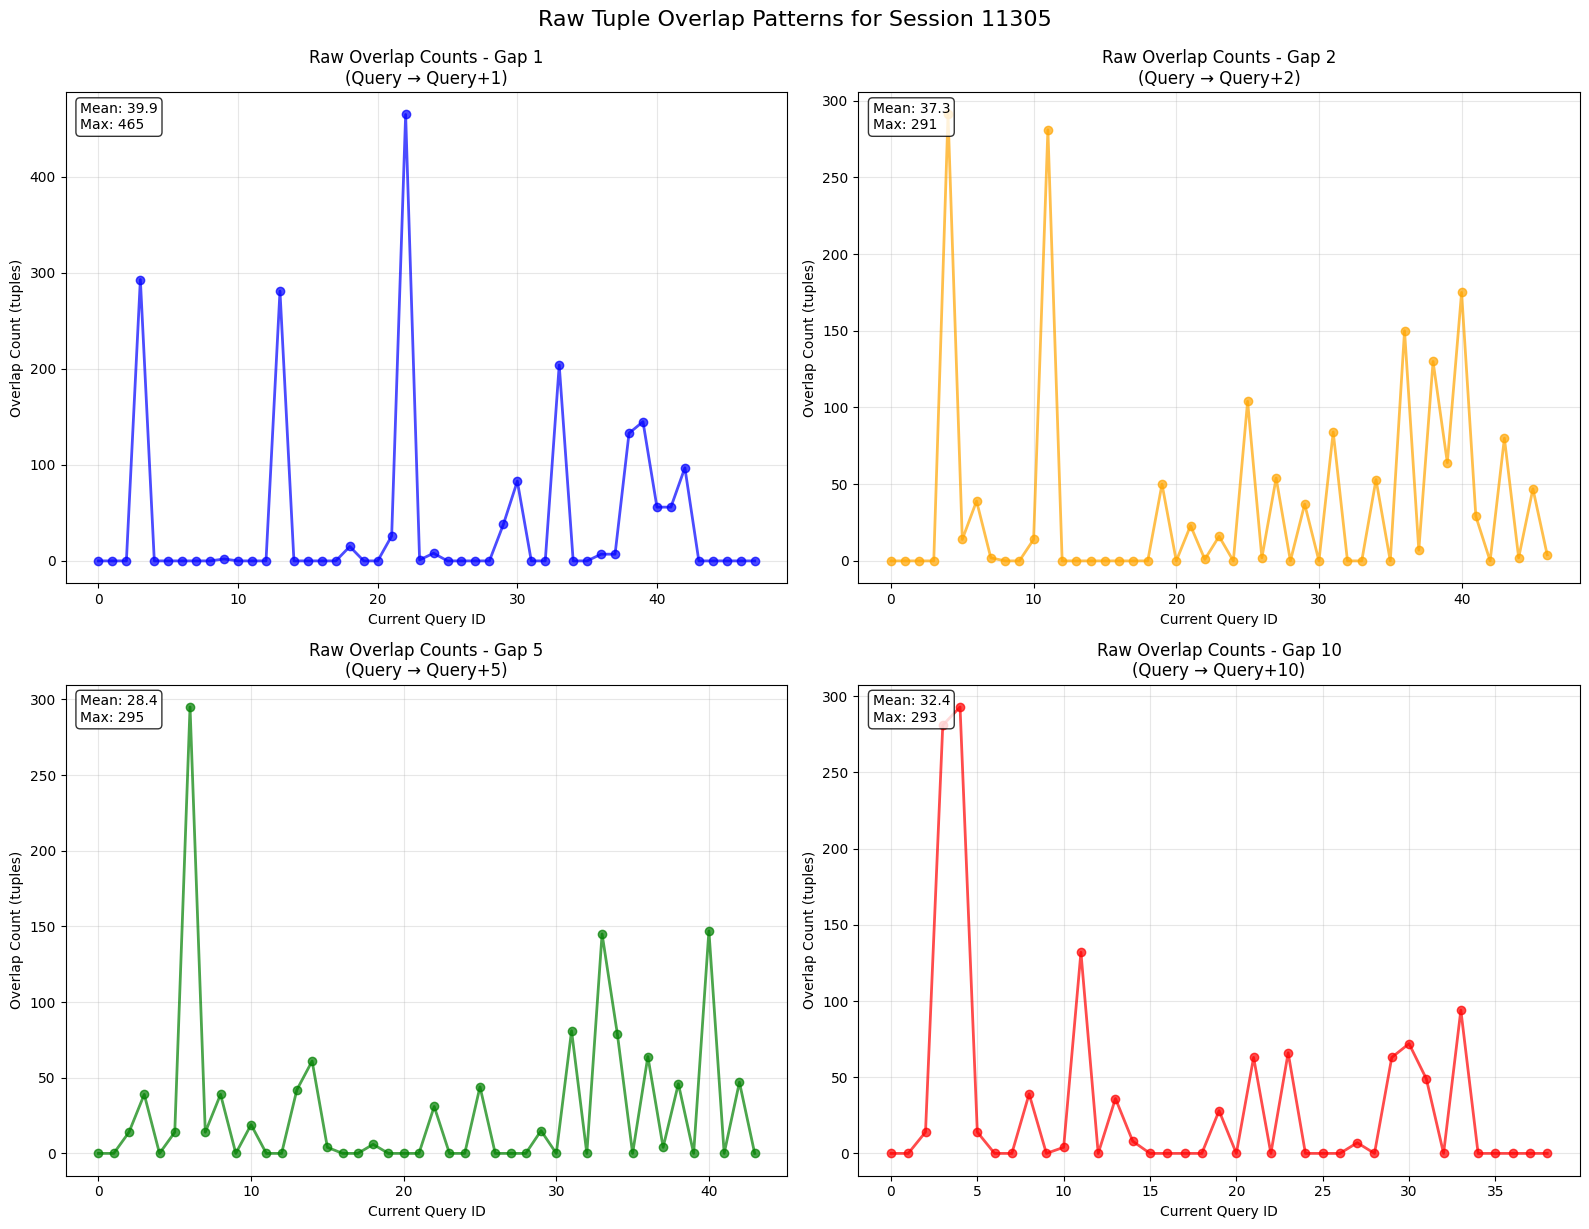
\includegraphics[scale=0.2]{figures/Overlap-analysis.png} 
\end{figure}

As such any kind of recommender needs to have a memory of what the user has already seen and be able to adapt to the user's changing interests. as such our reccomender keeps a memory of all results the user has looked at.

\textbf{Iterative Rule Maintenance.} Our system maintains a persistent set of association rules and summaries across exploration sessions, enabling the accumulation of knowledge about user interests over time. At each iteration, newly discovered patterns from current query results are combined with historical patterns to provide a comprehensive view of user preferences. Rules and summaries are weighted by recency and relevance, with older patterns gradually decaying in influence while frequently reinforced patterns maintain their strength.

The system employs a rule management strategy that balances memory efficiency with predictive accuracy. Rules that consistently fail to contribute to accurate predictions are pruned from the active set, while high-performing patterns are retained and strengthened. This approach ensures that the system adapts to evolving user interests while maintaining computational efficiency as exploration sessions progress.

\textbf{System Algorithm.} The complete system operates according to the following iterative process:

\begin{algorithmic}[1]
\Procedure{RecommendTuples}{$Q_{current}$, $R_{historical}$, $S_{historical}$}
    \State $T_{results} \gets$ \textsc{ExecuteQuery}($Q_{current}$)
    \State $F \gets$ \textsc{MineFrequentItemsets}($T_{results}$)
    \State $R_{new} \gets$ \textsc{MineAssociationRules}($F$)
    \State $S_{new} \gets$ \textsc{ApplyBUSSummarization}($T_{results}$)
    \State $R_{combined} \gets R_{historical} \cup R_{new}$
    \State $S_{combined} \gets S_{historical} \cup S_{new}$
    \For{each tuple $t \in T_{results}$}
        \State $I(t) \gets$ \textsc{ComputeInterestingness}($t$, $R_{combined}$, $S_{combined}$)
    \EndFor
    \State $T_{recommended} \gets$ \textsc{RankTuples}($T_{results}$, $I$)
    \State $R_{relevant} \gets$ \textsc{FilterRelevantRules}($R_{combined}$, $T_{recommended}$)
    \State $S_{relevant} \gets$ \textsc{FilterRelevantSummaries}($S_{combined}$, $T_{recommended}$)
    \State \Return $T_{recommended}$, $R_{relevant}$, $S_{relevant}$
\EndProcedure
\end{algorithmic}

where \textsc{ComputeInterestingness} applies the combined scoring formula from Equation (1), \textsc{RankTuples} orders tuples by decreasing interestingness score, and the filtering functions retain only rules and summaries that contribute to high-scoring tuples for the next iteration.






\section{Experimental Evaluation}

We consider a small sample of sessions SDSS that have 

\section{Related work}

\textbf{Query-by-Example and Interactive Data Exploration.} Existing data exploration systems rely heavily on explicit user interaction to guide the exploration process. Query-by-Example (QBE) approaches require users to provide explicit examples or feedback to formulate queries, demanding cognitive effort that interrupts the exploratory workflow. Interactive data exploration systems have proposed various explicit feedback mechanisms: YMALDB \cite{drosouYmaldbExploringRelational2013} recommends data similar to query results based on explicit user preferences; DICE uses faceted search requiring explicit facet selection; and systems like \cite{kalininInteractiveDataExploration2014} propose drill-down operators and semantic windows that require explicit user-driven navigation decisions. Query steering approaches \cite{ugurcetintemelQuerySteeringInteractive2013} and interactive query specification systems similarly demand explicit user feedback during query formulation.

\textbf{Query Relaxation and Refinement.} Query relaxation techniques focus on modifying query parameters to satisfy cardinality constraints or obtain non-empty results, but operate orthogonally to understanding user interests. These approaches employ explicit user acceptance/rejection of query modifications rather than inferring intent from exploration patterns. Unlike these systems that require users to explicitly evaluate and approve query modifications, our implicit feedback approach infers user interests from the natural progression of their exploration session, capturing intent through the organic evolution of their analytical investigation.

\textbf{Active Learning for Data Exploration.} Traditional active learning approaches maximize learning outcomes while minimizing labeled samples, but assume either small datasets or negligible sample extraction costs—assumptions that break down with large-scale data exploration. Relevance feedback techniques from information retrieval are designed for specific data types and do not optimize for efficient data space exploration in analytical contexts. These active learning paradigms require explicit user labeling of samples, creating cognitive overhead that disrupts the exploratory thought process.

\textbf{Collaborative Query Systems.} Collaborative approaches facilitate SQL query formulation based on past queries or provide query recommendations, but do not predict user interests from behavioral patterns. Query clustering techniques focus on understanding intent in web search contexts rather than structured database exploration. These collaborative systems assume static, predefined notions of similarity and do not adapt to individual user exploration patterns in real-time.

\textbf{Implicit Feedback in Recommendation Systems.} While implicit feedback has been extensively studied in traditional recommendation systems, its application to Exploratory Data Analysis (EDA) remains unexplored. Early work by Oh et al. \cite{oh2008user} proposed multi-criteria rating systems using implicit feedback for e-commerce applications, relying on ID3 decision trees for attribute importance determination with predefined product attributes. Recent advances have tackled exposure bias and missing data problems: Wang et al. \cite{wang2018modeling} introduced H4MF using Hidden Markov Models to capture temporal dependencies in user behavior for dynamic missingness modeling; Lin et al. \cite{lin2024recrec} proposed ReCRec, which reasons about causes behind implicit feedback by categorizing unclicked data into unexposed, dislike, or combination scenarios; and Wang et al. \cite{wang2021denoising} focused on denoising implicit feedback through Adaptive Denoising Training (ADT), achieving 15-21\% performance improvements by removing false positives. Wu et al. \cite{wu2022adapting} introduced Triplet Importance Learning (TIL) with bilevel optimization to adaptively weight training triplets in pairwise ranking, addressing the limitation that traditional methods treat all triplets equally. Guo and Huang \cite{guo2023implicit} developed sequence recommendation using Transformers for interactive interest modeling to capture real-time user interests through behavior sequences. Li et al. \cite{li2025beyond} identified "intentional implicit feedback" through user studies on social media platforms, revealing that users strategically employ behaviors to influence algorithmic recommendations.

All existing implicit feedback approaches focus on recommendation scenarios with predefined item catalogs, stable user preferences, consumption-oriented goals, and satisfaction-based success metrics—assumptions that are differnt to EDA, where the "item space" is dynamically generated through analytical operations, user interests evolve rapidly based on discovered insights, success is measured by knowledge discovery rather than satisfaction, and recommendations target analytical operations rather than content items. Our approach fundamentally differs from these explicit feedback paradigms by leveraging implicit signals from users' natural exploration behavior—specifically the sequence and characteristics of follow-up queries—eliminating the need for disruptive explicit feedback while maintaining exploration momentum. To the best of our knowledge, no prior work has addressed implicit recommendation specifically for EDA or SQL-based data exploration.

\section{Conclusion and Future Work}

This proof of concept system is limited in that it only looks at tuples the user looks at. This makes it very effective for drill-down or zooming like workloads but not as helpful for more general exploration. Future work will look at automated exploration of the database and modelling potential query trajectories.

\begin{acks}
\end{acks}

%\clearpage

\bibliographystyle{ACM-Reference-Format}
\bibliography{references}

\end{document}
\endinput
